\documentclass[../../main]{subfiles}
\begin{document}

\subsection{Compilatore SimplanPlus}
Il compilatore può essere eseguito tramite il comando \textit{java -jar SimplanPlus.jar [nomefile]} il quale si occuperà di:
\begin{itemize}
    \item Controllare errori lessicali;
    \item Controllare errori semantici;
    \item Controllare errori di tipo;
    \item Controllare errori di effetto;
    \item Compilare il codice in bytecode;
    \item Eseguire il bytecode generato;
\end{itemize}

Quindi \textit{compile(String fileAbsoluteName, String fileName)} si occupa di controllare tutti gli errori di tipo e nel caso non vi siano presenti
genera il bytecode e lo salva nell'apposita cartella. Da qui subentra \textit{interpreter(Instruction[] code,String filename)} che riceve il bytecode 
e lo esegue sulla VM.
\begin{figure}[H]
    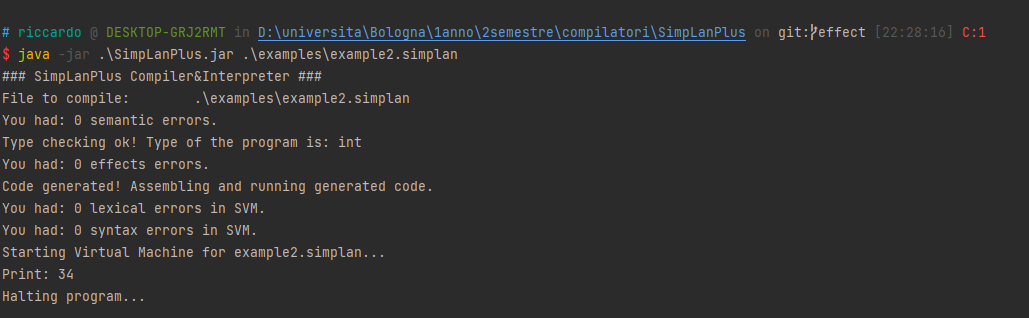
\includegraphics[width=170mm,height=70mm]{images/esempioesec.png}
    \caption{Esempio di esecuzione di un file.}
\end{figure}
\end{document}